\documentclass[tikz,border=2pt]{standalone}
\usepackage[utf8]{inputenc}
\begin{document}
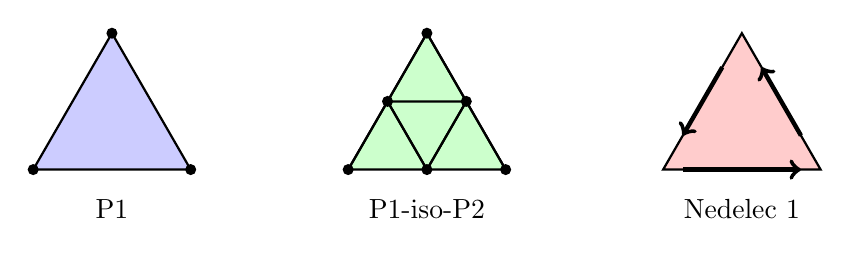
\begin{tikzpicture}

    % P1 Element - Filled
    \begin{scope}[shift={(0,0)}]
        \filldraw[fill=blue!20, draw=black, thick] (0,0) -- (2,0) -- (1,1.732) -- cycle;
        \foreach \p in {(0,0), (2,0), (1,1.732)} \fill[black] \p circle (2pt);
        \node at (1,-0.5) {P1};
    \end{scope}

    % P1-iso-P2 Element - Filled
    \begin{scope}[shift={(4,0)}]
        \filldraw[fill=green!20, draw=black, thick] (0,0) -- (2,0) -- (1,1.732) -- cycle;
        \draw[draw=black, thick] (1,0) -- (1.5,0.866) -- (0.5,0.866) -- cycle;
        \draw[draw=black, thick] (0,0) -- (0.5,0.866);
        \draw[draw=black, thick] (2,0) -- (1.5,0.866);
        \draw[draw=black, thick] (1,1.732) -- (0.5,0.866);
        \draw[draw=black, thick] (1,1.732) -- (1.5,0.866);
        \draw[draw=black, thick] (1,0) -- (0.5,0.866);
        \draw[draw=black, thick] (1,0) -- (1.5,0.866);
        \foreach \p in {(0,0), (2,0), (1,1.732), (1,0), (0.5,0.866), (1.5,0.866)} \fill[black] \p circle (2pt);
        \node at (1,-0.5) {P1-iso-P2};
    \end{scope}

    % Nédélec (1st kind) Element - Filled
    \begin{scope}[shift={(8,0)}]
        \filldraw[fill=red!20, draw=black, thick] (0,0) -- (2,0) -- (1,1.732) -- cycle;
        % Vectors centered along the edges, always black
        \draw[->, ultra thick, black] (0.25, 0) -- (1.75, 0);
        \draw[->, ultra thick, black] (1.75, 0.433) -- (1.25, 1.299);
        \draw[->, ultra thick, black] (0.75, 1.299) -- (0.25, 0.433);
        \node at (1,-0.5) {Nedelec 1};
    \end{scope}

\end{tikzpicture}
\end{document}
